% Suggested filename: כלל_יד_ימין_בפיזיקה.tex
\documentclass[12pt]{article}

%========== (1) Math Packages ==========
\usepackage{amsmath,amssymb,amsthm}

%========== (2) General Packages: Hebrew support, fonts, etc ==========
\usepackage{xcolor}
\usepackage{float}
\usepackage{graphicx}
\usepackage{hyperref}
\usepackage{booktabs}
\usepackage{enumerate}
\usepackage{fancyvrb}
\usepackage{fancyhdr}
\usepackage{setspace}
\usepackage[most]{tcolorbox}

\usepackage{fontspec}
\usepackage{polyglossia}

\newcommand{\enquote}[1]{\textquotedblleft #1\textquotedblright}

% Language settings
\setdefaultlanguage{hebrew}
\setotherlanguage{english}

% Fonts
% Ensure these fonts are installed on your system
\newfontfamily\hebrewfont[Script=Hebrew]{David CLM} % Or another preferred Hebrew font like Ezra SIL, Frank Ruehl CLM, etc.
\newfontfamily\englishfont{Times New Roman} % Or another preferred English font
\newfontfamily\hebrewfonttt[Script=Hebrew]{David CLM} % Monospace font for Hebrew if needed, can be same as hebrewfont

% Hyperref link color settings
\hypersetup{
  colorlinks=true,
  linkcolor=black, % Consistent with professional look
  urlcolor=black, % Consistent with professional look
  citecolor=black % Consistent with professional look
}

%========== Spacing and Paragraphs ==========
\onehalfspacing
\setlength{\parskip}{6pt} % Space between paragraphs
\setlength{\parindent}{0pt} % No paragraph indentation

%========== Header/Footer Settings ==========
\pagestyle{fancy}
\setlength{\headheight}{14.5pt} % Adjust if needed based on font size/header content
\addtolength{\topmargin}{-2.5pt} % Fine-tune top margin
\fancyhf{} % Clear header/footer
\lhead{} % Empty left header
\rhead{\today} % Date on the right header
\cfoot{\thepage} % Page number in the center footer
\renewcommand{\headrulewidth}{0.4pt} % Header line
\renewcommand{\footrulewidth}{0.4pt} % Footer line

%========== tcolorbox Setup ==========
% Adjusted colors for more saturated but soft look
\tcbset{
  boxsep=5pt,
  top=5pt, bottom=5pt, left=5pt, right=5pt,
  middle=5pt,
  sharp corners, % Consistent style
  enhanced, % Allows for more features like opacity, etc.
  breakable % Allows boxes to break across pages
}

%========== Special Boxes: Definition, Remark, Example ==========
\newtcolorbox{definitionBox}[1]{
  title=#1,
  colback=teal!10!white, % Soft teal background
  colframe=teal!70!black, % More saturated teal frame
  fonttitle=\bfseries,
  coltitle=black % Title color
}

\newtcolorbox{remarkBox}[1]{
  title=#1,
  colback=orange!10!white, % Soft orange background
  colframe=orange!70!black, % More saturated orange frame
  fonttitle=\bfseries,
  coltitle=black % Title color
}

\newtcolorbox{exampleBox}[1]{
  title=#1,
  colback=red!10!white, % Soft red/pink background
  colframe=red!70!black, % More saturated red frame
  fonttitle=\bfseries,
  coltitle=black % Title color
}

% Bullet fix for Hebrew lists
\renewcommand{\labelitemi}{$\bullet$}

% Table of Contents customization (as provided)
\usepackage{tocloft}
\usepackage{etoolbox}
\makeatletter
\renewcommand\tableofcontents{\section*{ \contentsname}
    @starttoc{toc}}
\makeatother
% Ensure \contentsname is defined correctly for Hebrew - polyglossia handles this.

% Disable specific warnings if necessary, e.g., about hyperref/tcolorbox interaction
\RequirePackageWithOptions{tcolorbox}

\begin{document}

\begin{center}
    \Huge\textbf{כלל יד ימין בפיזיקה} \\
    \Large מדריך פשוט לשימוש בקביעת כיוונים בשדות מגנטיים
\end{center}

\vspace{1cm}

\tableofcontents

\newpage % Start content on a new page

\section{מבוא}
כלל יד ימין הוא כלי עזר ויזואלי שימושי וחיוני בפיזיקה, במיוחד בתחומי החשמל והמגנטיות. הוא מאפשר לנו לקבוע בקלות את הכיוון של גדלים וקטוריים כמו כוחות, שדות מגנטיים ומומנטים, כאשר ידועים הכיוונים של גדלים וקטוריים אחרים המעורבים במערכת. כלל זה מבוסס על ההגדרה הגיאומטרית של מכפלה וקטורית (\( \vec{A} \times \vec{B} \)), שתוצאתה היא וקטור המאונך לשני הווקטורים המוכפלים. כיוונו של הווקטור התוצאה נקבע על פי כלל יד ימין.

\section{העיקרון הבסיסי של כלל יד ימין}
כלל יד ימין משמש למציאת הכיוון של וקטור הנוצר ממכפלה וקטורית של שני וקטורים אחרים. באופן כללי, אם יש לנו שני וקטורים \( \vec{A} \) ו-\( \vec{B} \), והווקטור \( \vec{C} \) מוגדר כמכפלה הווקטורית שלהם:
\[ \vec{C} = \vec{A} \times \vec{B} \]
אז הכיוון של \( \vec{C} \) נקבע לפי כלל יד ימין:

\begin{definitionBox}{כלל יד ימין (גרסה כללית)}
כדי למצוא את הכיוון של \( \vec{C} = \vec{A} \times \vec{B} \):
\begin{itemize}
    \item הושיטו את יד ימין כאשר האצבעות ישרות בכיוון הווקטור הראשון (\( \vec{A} \)).
    \item סובבו את היד כך שתוכלו לכופף את האצבעות לכיוון הווקטור השני (\( \vec{B} \)) דרך הזווית הקטנה יותר בין הווקטורים.
    \item האגודל של יד ימין יצביע כעת בכיוון הווקטור התוצאה (\( \vec{C} \)).
\end{itemize}
\end{definitionBox}

\begin{remarkBox}{הערה חשובה}
סדר הווקטורים במכפלה הווקטורית קריטי. המכפלה \( \vec{B} \times \vec{A} \) תיתן וקטור בעל אותו גודל אך בכיוון הפוך מ-\( \vec{A} \times \vec{B} \). שימוש בכלל יד ימין דורש לשמור על הסדר הנכון.
\end{remarkBox}

\section{יישומים נפוצים של כלל יד ימין}

כלל יד ימין מופיע בפורמולציות רבות בפיזיקה, בעיקר במגנטיות. נציג כאן שני יישומים עיקריים.

\subsection{שדה מגנטי מחוט נושא זרם}

זרם חשמלי העובר בחוט מוליך יוצר סביבו שדה מגנטי. כיוונו של השדה המגנטי בנקודה מסוימת תלוי בכיוון הזרם ובמיקום הנקודה ביחס לחוט. כלל יד ימין מספק דרך קלה לקבוע כיוון זה.

\begin{definitionBox}{כלל יד ימין לשדה מגנטי מחוט נושא זרם}
כדי לקבוע את כיוון השדה המגנטי (\( \vec{B} \)) סביב חוט ישר נושא זרם (\( I \)):
\begin{itemize}
    \item אחזו בחוט המוליך ביד ימין.
    \item מקמו את האגודל בכיוון הזרם החשמלי (\( I \)).
    \item כיוון האצבעות העוטפות את החוט מצביע על כיוון קווי השדה המגנטי סביב החוט. קווי השדה יהיו מעגלים סביב החוט.
\end{itemize}
\end{definitionBox}

\begin{figure}[H]
  \centering
  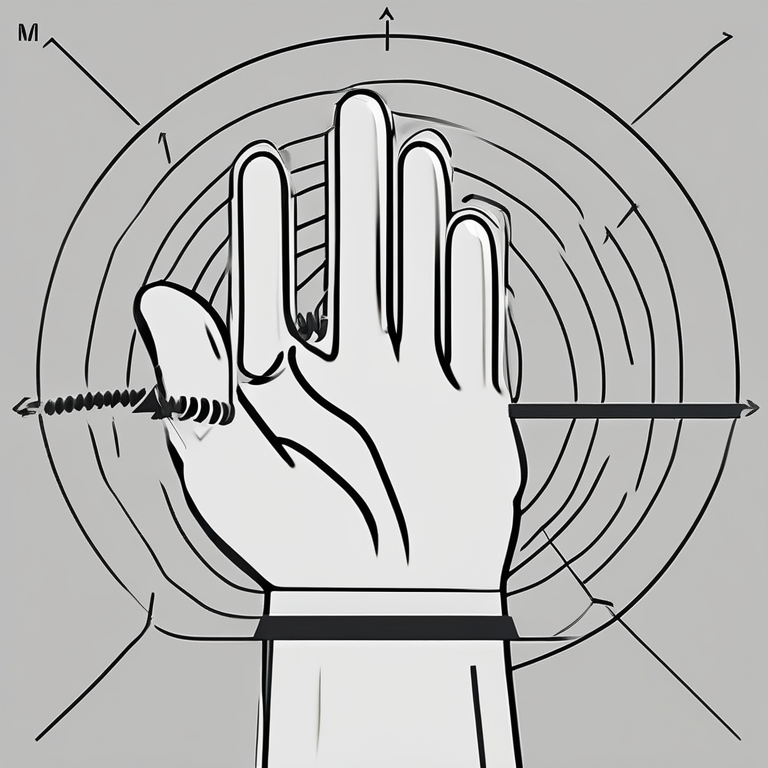
\includegraphics[width=0.6\textwidth]{files/right_hand_rule_diagram.png}
  \caption{איור המתאר את כלל יד ימין לקביעת כיוון השדה המגנטי סביב חוט נושא זרם ישר. האגודל מצביע בכיוון הזרם, והאצבעות העוטפות מצביעות על כיוון קווי השדה המגנטי.}
\end{figure}

עבור חוט ארוך וישר, גודל השדה המגנטי במרחק \( r \) מהחוט נתון על ידי:
\[ B = \frac{\mu_0 I}{2\pi r} \]
כאשר \( \mu_0 \) היא פרמיאביליות הריק.

\subsection{כוח לורנץ על מטען נע בשדה מגנטי}

מטען חשמלי הנע בתוך שדה מגנטי חווה כוח מגנטי, המכונה כוח לורנץ. כיוון הכוח תלוי בסימן המטען, כיוון מהירותו וכיוון השדה המגנטי.

\begin{definitionBox}{כוח לורנץ}
הכוח המגנטי (\( \vec{F} \)) הפועל על מטען חשמלי (\( q \)) הנע במהירות (\( \vec{v} \)) בשדה מגנטי (\( \vec{B} \)) נתון על ידי הנוסחה:
\[ \vec{F} = q (\vec{v} \times \vec{B}) \]
\end{definitionBox}

כיוון הכוח \( \vec{F} \) נקבע באמצעות כלל יד ימין על המכפלה הווקטורית \( \vec{v} \times \vec{B} \).

\begin{definitionBox}{כלל יד ימין לכוח לורנץ}
כדי לקבוע את כיוון כוח לורנץ (\( \vec{F} \)) הפועל על מטען \( q \) הנע במהירות \( \vec{v} \) בשדה מגנטי \( \vec{B} \):
\begin{itemize}
    \item הושיטו את יד ימין כאשר האצבעות ישרות בכיוון וקטור המהירות (\( \vec{v} \)).
    \item סובבו את היד כך שתוכלו לכופף את האצבעות לכיוון וקטור השדה המגנטי (\( \vec{B} \)) דרך הזווית הקטנה יותר.
    \item האגודל של יד ימין יצביע כעת בכיוון המכפלה הווקטורית \( \vec{v} \times \vec{B} \).
    \item אם המטען \( q \) חיובי, כיוון הכוח \( \vec{F} \) זהה לכיוון \( \vec{v} \times \vec{B} \).
    \item אם המטען \( q \) שלילי, כיוון הכוח \( \vec{F} \) הפוך לכיוון \( \vec{v} \times \vec{B} \). במקרה זה, לאחר מציאת הכיוון עבור מטען חיובי, יש להפוך את הכיוון. ניתן גם להשתמש ביד שמאל, אך מקובל יותר פשוט להשתמש ביד ימין ולהפוך את התוצאה למטען שלילי.
\end{itemize}
\end{definitionBox}

\subsection{כוח מגנטי על מוליך נושא זרם בשדה מגנטי}

יישום נוסף של כוח לורנץ הוא הכוח הפועל על קטע חוט נושא זרם המוצב בשדה מגנטי. ניתן לחשוב על הזרם כעל תנועה מסודרת של מטענים בתוך המוליך.

\begin{definitionBox}{כוח מגנטי על מוליך נושא זרם}
הכוח המגנטי (\( \vec{F} \)) הפועל על קטע מוליך באורך \( \vec{L} \) (וקטור בכיוון הזרם) שדרכו עובר זרם \( I \) המוצב בשדה מגנטי חיצוני (\( \vec{B} \)) נתון על ידי:
\[ \vec{F} = I (\vec{L} \times \vec{B}) \]
\end{definitionBox}

כיוון הכוח \( \vec{F} \) נקבע באמצעות כלל יד ימין על המכפלה הווקטורית \( \vec{L} \times \vec{B} \). במקרה זה, האצבעות תחילה יצביעו בכיוון הזרם (\( \vec{L} \)), יתכופפו לכיוון השדה המגנטי (\( \vec{B} \)), והאגודל יצביע לכיוון הכוח (\( \vec{F} \)).

\section{סיכום}
כלל יד ימין הוא כלי גיאומטרי פשוט אך רב עוצמה לפיזיקאים ומהנדסים, המאפשר לקבוע כיוונים במערכות תלת-ממדיות המערבות מכפלות וקטוריות. זכרו את היישומים העיקריים שלו: קביעת כיוון השדה המגנטי סביב חוט נושא זרם (אגודל=זרם, אצבעות=שדה), וקביעת כיוון כוח לורנץ (אצבעות=מהירות, כיפוף=שדה, אגודל=כוח, תוך התחשבות בסימן המטען). שליטה בכלל זה חיונית להבנה אינטואיטיבית ולפתרון בעיות בתחומי החשמל והמגנטיות.

\end{document}